% This is auto-generated file: do not edit!
% Exported from microMathematics Plus, version 2.20.0


Dieses Beispiel zeigt, wie Sie Reihen
und Integrale berechnen können.

\subsection{Taylor Reihe}

In der Mathematik ist die Taylor Reihe
eine Repräsentation einer Funktion als
unendliche Summe von Termen, die von
den Werten der Ableitung dieser
Funktion an einem bestimmten Punk
berechnet werden.

Beispielsweise ist Ts(x,N) die
Taylorentwicklung als Funktion des
Arguments x und der Anzahl von N
Termen:
\begin{center}\begin{tabular}{c}
  $Ts(x,N) := \displaystyle\sum_{n=0}^{N} \frac{{ \left( -1\right) }^{n}}{\left( 2 \cdot n \right)! } \cdot {x}^{2 \cdot n}$
\end{tabular}\end{center}

Diese Entwicklung nähert sich der
Kosinus-Funktion an:
\begin{center}\begin{tabular}{c}
  $s(x) := cos \left( x\right) $
\end{tabular}\end{center}

Wenn wir beide Funktionen für das selbe
Intervall auftragen, so sehen beide
gleich aus: 
\begin{center}\begin{tabular}{c}
  $x := \left[ 0,\, 0.1 \,..\, 2 \cdot {\pi} \right]$
\end{tabular}\end{center}
\begin{center}\begin{tabular}{c} 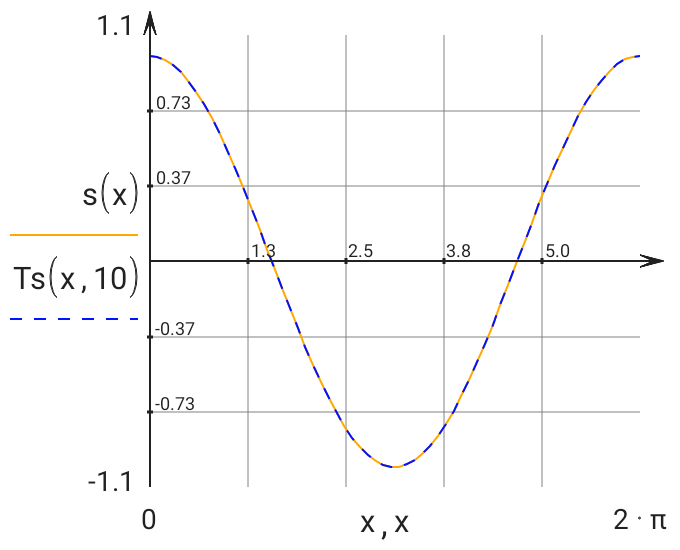
\includegraphics[width=0.45\textwidth]{graphics/series_and_integrals_fig1.png} \end{tabular}\end{center}

Jedoch ist dies ein numerischer Fehler,
der aus der eingeschränkten Anzahl von
Annäherungstermen N resultiert. Die
folgende Funktion $\Delta$(x,N) beschreibt
diesen Fehler:
\begin{center}\begin{tabular}{c}
  ${\Delta}(x,N) :=  \left| s \left( x\right)  - Ts \left( x,\, N\right)  \right| $
\end{tabular}\end{center}

Wir können diese Funktion in
logarithmischen Koordinaten ausdrücken
und werden sehen, dass der numerische
Fehler sich verringert hat, wenn wir
mehr Terme in die Taylorreihe
integrieren:
\begin{center}\begin{tabular}{c}
  $N := \left[ 3,\, 4 \,..\, 13 \right]$
\end{tabular}\end{center}
\begin{center}\begin{tabular}{c} 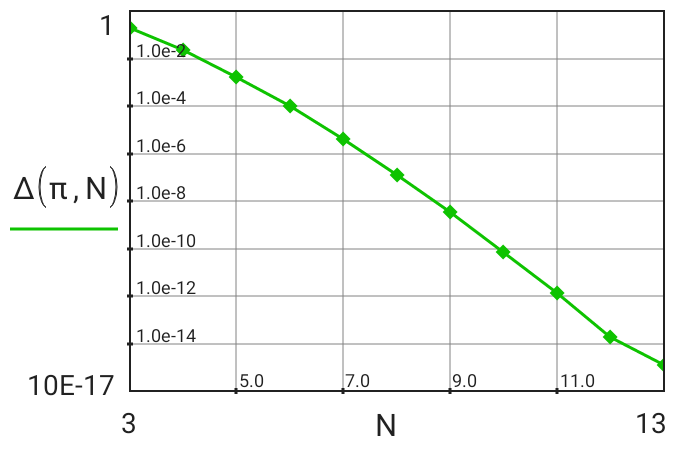
\includegraphics[width=0.45\textwidth]{graphics/series_and_integrals_fig2.png} \end{tabular}\end{center}

\subsection{Binomische Reihen}

Betrachten wir diese Potenzfunktion:
\begin{center}\begin{tabular}{c}
  $f(x,{\alpha}) := {\left( 1 + x \right)}^{{\alpha}}$
\end{tabular}\end{center}

Dieser Funktion kann sich durch eine
Binomische Reihe angenähert werden:
\begin{center}\begin{tabular}{c}
  $Tf(x,{\alpha},N) := \displaystyle\sum_{n=0}^{N}  \left( \displaystyle\prod_{k=1}^{n} \frac{{\alpha} - k + 1}{k}\right)  \cdot {x}^{n}$
\end{tabular}\end{center}

Zudem können wir beide Funktionen (die
gegebene Potenzfunktion und ihre
Annäherung) im gleichen Plot
auftragen:
\begin{center}\begin{tabular}{c} 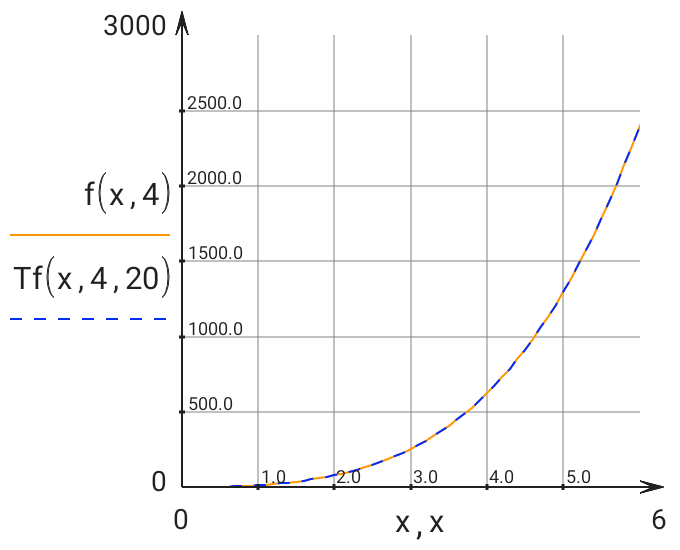
\includegraphics[width=0.45\textwidth]{graphics/series_and_integrals_fig3.png} \end{tabular}\end{center}

\subsection{Integrale}

Außerdem ist es möglich, ein
bestimmtes Integral mittels der
Simpson Methode numerisch zu
berechnen. Beispielsweise können wir
das Integral durch das Element
''Ergebnisansicht'' berechnen:
\begin{center}\begin{tabular}{c}
  $\displaystyle\int_{0}^{3 \cdot pi / 2}{cos \left( \frac{2 \cdot x}{9}\right) }^{-2}\, dx = 7.79423$
\end{tabular}\end{center}

Das analytische Ergebnis ist
\begin{center}\begin{tabular}{ccc}
  $I := \frac{9 \cdot \sqrt{3} }{2}$ &
  ,    &
  $I = 7.79423$ \cr
\end{tabular}\end{center}

Der numerische Fehler kann wie folgt
berechnet werden:
\begin{center}\begin{tabular}{c}
  $\displaystyle\int_{0}^{3 \cdot pi / 2}{cos \left( \frac{2 \cdot x}{9}\right) }^{-2}\, dx - I = 4.26681E-9$
\end{tabular}\end{center}

Dieser Fehler hängt von dem Wert
''Signifikante Ziffern im Ergebnis'' ab,
was in den ''Dokumenteinstellungen''
Dialog verändert werden kann:
\begin{center}\begin{tabular}{c} 
\includegraphics[width=0.45\textwidth]{graphics/series_and_integrals_fig4.png} \end{tabular}\end{center}

Wird dieser Wert erhöht, so erhöht sich
auch die Grenze, welche die
Genauigkeit der Simpson Methode
kontrolliert.